\documentclass{article}
\usepackage[backend=biber,natbib=true,style=alphabetic,maxbibnames=50]{biblatex}
\addbibresource{/home/nqbh/reference/bib.bib}
\usepackage[utf8]{vietnam}
\usepackage{tocloft}
\renewcommand{\cftsecleader}{\cftdotfill{\cftdotsep}}
\usepackage[colorlinks=true,linkcolor=blue,urlcolor=red,citecolor=magenta]{hyperref}
\usepackage{amsmath,amssymb,amsthm,enumitem,float,graphicx,mathtools,tikz}
\usetikzlibrary{angles,calc,intersections,matrix,patterns,quotes,shadings}
\allowdisplaybreaks
\newtheorem{assumption}{Assumption}
\newtheorem{baitoan}{Bài toán}
\newtheorem{cauhoi}{Câu hỏi}
\newtheorem{conjecture}{Conjecture}
\newtheorem{corollary}{Corollary}
\newtheorem{dangtoan}{Dạng toán}
\newtheorem{definition}{Definition}
\newtheorem{dinhly}{Định lý}
\newtheorem{dinhnghia}{Định nghĩa}
\newtheorem{example}{Example}
\newtheorem{ghichu}{Ghi chú}
\newtheorem{hequa}{Hệ quả}
\newtheorem{hypothesis}{Hypothesis}
\newtheorem{lemma}{Lemma}
\newtheorem{luuy}{Lưu ý}
\newtheorem{nhanxet}{Nhận xét}
\newtheorem{notation}{Notation}
\newtheorem{note}{Note}
\newtheorem{principle}{Principle}
\newtheorem{problem}{Problem}
\newtheorem{proposition}{Proposition}
\newtheorem{question}{Question}
\newtheorem{remark}{Remark}
\newtheorem{theorem}{Theorem}
\newtheorem{vidu}{Ví dụ}
\usepackage[left=1cm,right=1cm,top=5mm,bottom=5mm,footskip=4mm]{geometry}
\def\labelitemii{$\circ$}
\DeclareRobustCommand{\divby}{%
	\mathrel{\vbox{\baselineskip.65ex\lineskiplimit0pt\hbox{.}\hbox{.}\hbox{.}}}%
}
\setlist[itemize]{leftmargin=*}
\setlist[enumerate]{leftmargin=*}

\title{Lecture Note: Mathematics for Machine Learning\\Bài Giảng: Toán Học Cho Học Máy}
\author{Nguyễn Quản Bá Hồng\footnote{A Scientist {\it\&} Creative Artist Wannabe. E-mail: {\tt nguyenquanbahong@gmail.com}. Bến Tre City, Việt Nam.}}
\date{\today}

\begin{document}
\maketitle
\begin{abstract}
	This text is a part of the series {\it Some Topics in Advanced STEM \& Beyond}:
	
	{\sc url}: \url{https://nqbh.github.io/advanced_STEM/}.
	
	Latest version:
	\begin{itemize}
		\item {\it Lecture Note: Mathematics for Machine Learning}.
		
		PDF: {\sc url}: \url{https://github.com/NQBH/advanced_STEM_beyond/blob/main/machine_learning/lecture/NQBH_mathematics_for_machine_learning_lecture.pdf}.
		
		\TeX: {\sc url}: \url{https://github.com/NQBH/advanced_STEM_beyond/blob/main/machine_learning/lecture/NQBH_mathematics_for_machine_learning_lecture.tex}.
		\item {\it Slide: Mathematics for Machine Learning -- Toán Học cho Học Máy}.
		
		PDF: {\sc url}: \url{https://github.com/NQBH/advanced_STEM_beyond/blob/main/machine_learning/slide/NQBH_mathematics_for_machine_learning_slide.pdf}.
		
		\TeX: {\sc url}: \url{https://github.com/NQBH/advanced_STEM_beyond/blob/main/machine_learning/slide/NQBH_mathematics_for_machine_learning_slide.tex}.
		\item {\it Personal Expository Notes on Machine Learning}.
		
		PDF: {\sc url}: \url{https://github.com/NQBH/draft/blob/master/machine_learning/NQBH_machine_learning.pdf}.
		
		\TeX: {\sc url}: \url{https://github.com/NQBH/draft/blob/master/machine_learning/NQBH_machine_learning.tex}.
		\item Codes:
		\begin{itemize}
			\item Python for Machine Learning: \url{https://github.com/NQBH/advanced_STEM_beyond/tree/main/machine_learning/Python}.
			\item C{\tt/}C++ for Machine Learning:
		\end{itemize}
	\end{itemize}
\end{abstract}
\tableofcontents

%------------------------------------------------------------------------------%

\section{Basic \& Big Pictures}

\subsection{Abbreviation, Notations}

\begin{itemize}
	\item AI: Artificial Intelligence
	\item ANN: Artificial Neural Networks
	\item DL: Deep Learning
	\item ML: Machine Learning
\end{itemize}

\subsection{Main components}
\begin{figure}[H]
	\centering
	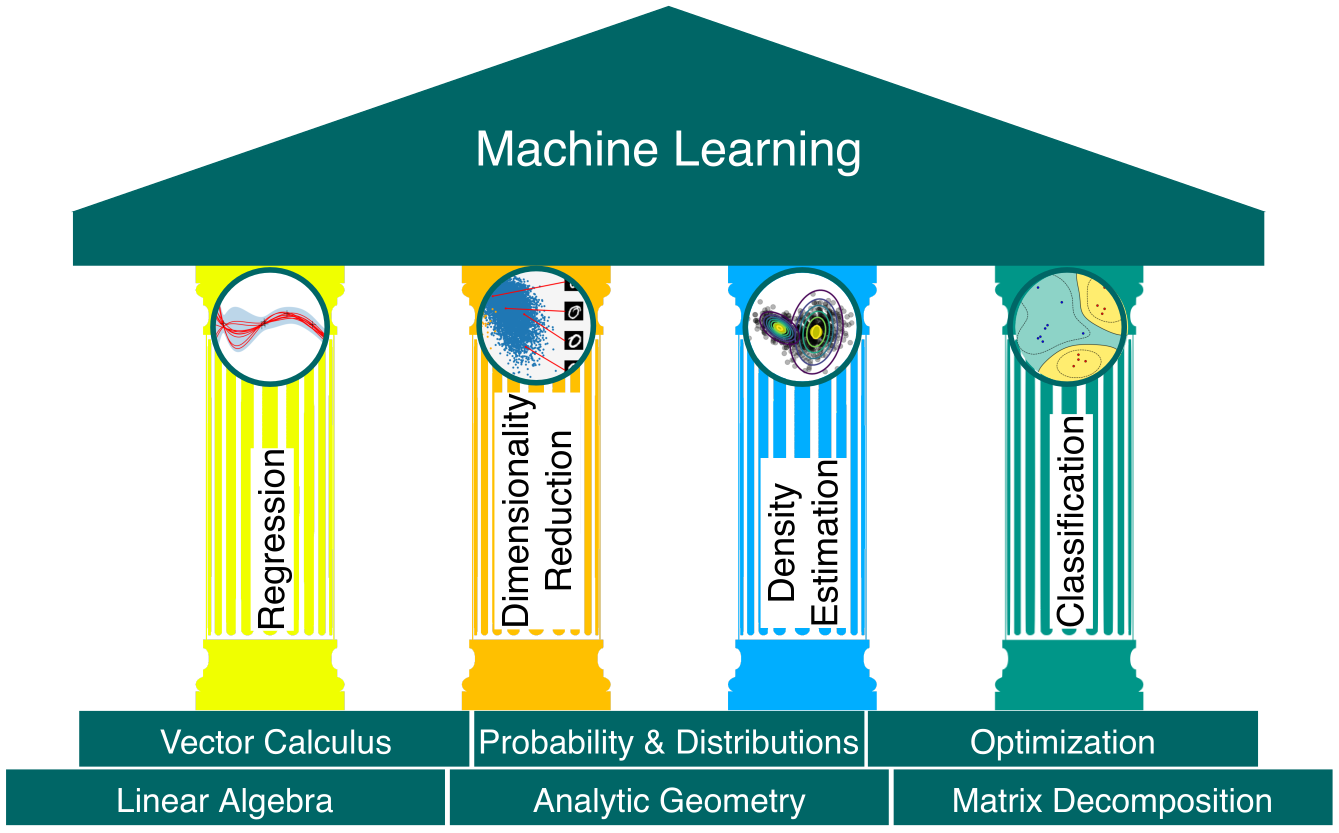
\includegraphics[width=12cm]{4_ML_pillars}
	\caption{Foundations \& 4 pillars of ML. Source: \cite[Fig. 1.1, p. 14]{Deisenroth_Faisal_Ong2024}.}
\end{figure}

\begin{itemize}
	\item 3 major components of a ML system: data, models, \& learning.
	\item 4 pillars of machine learning -- 4 trụ cột của máy học:
	\begin{enumerate}
		\item Regression -- Hồi quy
		\item Dimensionality reduction -- Giảm kích thước\footnote{I was used to work in project ROMSOC: Reduced Order Modelling, Simulation \& Optimization of Coupled Systems. Maybe ``dimensionality reduction'' is related to ``reduced order modeling'' in some sense of mathematics?}
		\item Density estimation -- Ước tính mật độ
		\item Classification -- Phân loại
	\end{enumerate}
\end{itemize}

\begin{question}[Main question of ML]
	What do we mean by ``good'' ``models''?
\end{question}
See, e.g., \cite[Chap. 8, Sect. 8.1: Data, Models, \& Learning]{Deisenroth_Faisal_Ong2024}.

\subsection{Data as vectors}
Input data can be considered as a vector of features of the problem considered.

See, e.g., \cite[Chap. 8, Sect. 8.1.1: Data as Vectors]{Deisenroth_Faisal_Ong2024}.

\subsection{How to describe models}
2 major approaches to describe models in ML:
\begin{itemize}
	\item a predictor as a function (i.e., non-probabilistic view of ML)
	\item a predictor as a probabilistic model (i.e., probabilistic view of ML).
\end{itemize}

\begin{remark}[Cf. Deterministic world vs. Stochastic world]
	
\end{remark}

\subsubsection{Models as functions -- Mô hình như hàm số}
See, e.g., \cite[Chap. 8, Sect. 8.1.2: Models as Functions]{Deisenroth_Faisal_Ong2024}.

A predictor is a function that, when given a particular input example produces an output:
\begin{align*}
	\mbox{predictor}:\mbox{Input Space}&\to\mbox{Output Space},\\
	\mbox{input example}&\mapsto\mbox{output}\coloneqq\mbox{predictor}(\mbox{input example}).
\end{align*}
Input- \& Output Spaces in this formula are usually vector spaces. If they are, we usually take $\mbox{Input Space}\coloneqq\mathbb{R}^{n_{\rm input}}$, $\mbox{Output Space}\coloneqq\mathbb{R}^{n_{\rm output}}$, or $\mbox{Input Space}\coloneqq\mathbb{C}^{n_{\rm input}}$, $\mbox{Output Space}\coloneqq\mathbb{C}^{n_{\rm output}}$, but each complex number can be decomposed as $z = \Re z + i\Im z$, $\forall z\in\mathbb{C}$, so it is equivalent to consider $\mbox{Input Space}\coloneqq\mathbb{R}^{2n_{\rm input}}$, $\mbox{Output Space}\coloneqq\mathbb{R}^{2n_{\rm output}}$ instead of $\mbox{Input Space}\coloneqq\mathbb{C}^{n_{\rm input}}$, $\mbox{Output Space}\coloneqq\mathbb{C}^{n_{\rm output}}$. Briefly, a pair of Euclidean spaces $(\mathbb{R}^{n_{\rm input}},\mathbb{R}^{n_{\rm output}})$ is good enough to represent input- \& output spaces. For simplicity, consider the output to be a single real number, i.e., a real-valued scalar output, which can be written as
\begin{equation*}
	f:\mathbb{R}^D\to\mathbb{R},
\end{equation*}
where the input vector ${\bf x}$ is $D$-dimensional (has $D$ features), \& the function $f$ then applied to it (written as $f({\bf x})$) returns a real number. In \cite{Deisenroth_Faisal_Ong2024}, the authors did not considered the general case of all functions, which would involve the need for functional analysis (see some classical texts of Functional Analysis, e.g., \cite{Alt2016,Brezis2011,Rudin1991}). Instead, they considered the special case of linear functions
\begin{equation}
	\label{linear predictor}
	\tag{linprd}
	f({\bf x}) = \boldsymbol{\theta}^\top{\bf x} + \theta_0 = \boldsymbol{\theta}\cdot{\bf x} + \theta_0 = \sum_{i=1}^D \theta_ix_i + \theta_0,\mbox{ also } f({\bf x}) = {\bf w}^\top{\bf x} + b = {\bf w}\cdot{\bf x} + b = \sum_{i=1}^D w_ix_i + b,
\end{equation}
for unknown $\boldsymbol{\theta},\theta_0$ (or more precisely, unknown but adjustable parameters) (or weights ${\bf w}$ \& bias $b$). The linear restriction of possible forms of predictors means that basic concepts of Linear Algebra \& Analytic Geometry suffice for precisely stating the notion of a predictor for the non-probabilistic view of machine learning. Linear functions strike a good balance between the generality of the problems that can be solved \& the amount of background mathematics, especially for computer science-major students, that is needed.

\begin{remark}[Pros \& cons of linear world vs. nonlinear world -- Ưu \& nhược điểm của thế giới tuyến tính so với thế giới phi tuyến tính]
	\item(i) Cf: Linear Functional Analysis vs. Nonlinear Functional Analysis.
	\item(ii) Cf: Linear Partial Differential Equations (linear PDEs) vs. Nonlinear Partial Differential Equations (nonlinear PDEs).
\end{remark}
Philosophically \& mathematically speaking, in any case, some compromises that are good enough are needed to be established for particular goals.

\subsubsection{Models as probability distributions -- Mô hình như phân phối xác suất}
See, e.g., \cite[Chap. 8, Sect. 8.1.3: Models as Probability Distributions]{Deisenroth_Faisal_Ong2024}.

We often consider data to be noisy observations of some true underlying effect, i.e.,
\begin{equation*}
	\mbox{noise data}\coloneqq\mbox{true data} + \mbox{noise},\ {\bf x}_{\rm noise}\coloneqq{\bf x}_{\rm true} + \delta_{\rm noise},
\end{equation*}
\& hope that by apply ML we can identity the signal from the noise (denoise), which requires
\begin{itemize}
	\item a language for quantifying the effect of noise (probability theory provides a language for quantifying uncertainty), \&
	\item predictors being able to express some sort of uncertainty, e.g., to quantify the confidence we have about the value of the prediction for a particular test data point.
\end{itemize}
{\sf Idea.} Instead of considering a predictor as a single function, we could consider predictors to be probabilistic models, i.e., models describing the distribution of possible functions. In \cite{Deisenroth_Faisal_Ong2024}, the authors limited themselves to the special case of distributions with finite-dimensional parameters, which allows them to describe probabilistic models without needing stochastic processes \& random measures. For this special case, we can think about probabilistic models as multivariate probability distributions, which already allow for a rich class of models.

\subsubsection{Learning is finding parameters}
See, e.g., \cite[Chap. 8, Sect. 8.1.4: Learning is Finding Parameters]{Deisenroth_Faisal_Ong2024}.

The goal of learning is to find a model \& its corresponding parameters such that the resulting predictor will perform well on unseen data. There are conceptually 3 distinct algorithmic phases when discussing ML algorithms:
\begin{enumerate}
	\item Prediction or inference -- Dự đoán hoặc suy luận
	\item Training or parameter estimation -- Đào tạo hoặc ước tính tham số
	\item Hyperparameter tuning or model selection -- Điều chỉnh siêu tham số hoặc lựa chọn mô hình
\end{enumerate}
The prediction phase is when we use a trained predictor on previously unseen test data, i.e., the parameters \& model choice is already fixed \& the predictor is applied to new vectors representing new input data points. Recall that we consider 2 schools of ML, corresponding to whether the predictor is a function or a probabilistic model. When we have a probabilistic model (see, e.g., \cite[Sect. 8.4]{Deisenroth_Faisal_Ong2024}) the prediction phase is called {\it inference}.

\begin{remark}[Usage of word ``inference'' -- Các cách sử dụng từ ``suy luận'']
	``Unfortunately, there is no agreed upon naming for different algorithmic phases. The word ``inference'' is sometimes also used to mean parameter estimation of a probabilistic model, \& less often may be also used to mean prediction for non-probabilistic models.'' -- \cite[Rmk, p. 257]{Deisenroth_Faisal_Ong2024})
	
	-- Thật không may, không có cách đặt tên thống nhất cho các giai đoạn thuật toán khác nhau. Từ ``suy luận'' đôi khi cũng được dùng để chỉ ước tính tham số của một mô hình xác suất, \& ít thường xuyên hơn có thể được dùng để chỉ dự đoán cho các mô hình không xác suất.
\end{remark}
We are interested in learning a model based on data s.t. it performs well on future data. It is not enough for the model to only fit the training data well, the predictor needs to perform well on unseen data. We simulate the behavior of our predictor on future unseen data using {\it cross-validation}. To check the goal of performing well on unseen data, we will need to balance between fitting well on training data \& finding ``simple'' explanations of the phenomenon. This trade-off is achieved using {\it regularization} or by {\it adding a prior}. In philosophy, this is considered to be neither induction nor deduction, but is called {\it abduction}. According to the {\it Stanford Encyclopedia of Philosophy, abduction} is the process of inference to the best explanation.

We often need to make high-level modeling decisions about the structure of the predictor, e.g. the number of components to use or the class of probability distributions to consider. The choice of the number of components is an example of a {\it hyperparameter}, \& this choice can affect the performance of the model significantly. The problem of choosing among different models is called {\it model selection} (see, e.g., \cite[Sect. 8.6: Model Selection]{Deisenroth_Faisal_Ong2024}). For non-probabilistic models, model selection is often done using {\it nested cross-validation} (see, e.g., \cite[Subsect. 8.6.1: Nested Cross-Validation]{Deisenroth_Faisal_Ong2024}). We also use model selection to choose hyperparameters of our model.

\begin{remark}[Cf. Parameter vs. Hyperparameter]
	The distinction between parameters \& hyperparameters is somewhat arbitrary, \& is mostly driven by the distinction between what can be numerically optimized vs. what needs to use search techniques. Another way to consider the distinction is to consider parameters as the explicit parameters of a probabilistic model, \& to consider hyperparameters (higher-level parameters) as parameters that control the distribution of these explicit parameters.
\end{remark}
3 flavors of ML:
\begin{enumerate}
	\item Empirical risk minimization, see, e.g., \cite[Sect. 8.2: Empirical Risk Minimization]{Deisenroth_Faisal_Ong2024};
	\item Principle of maximum likelihood, see, e.g., \cite[Sect. 8.3: Parameter Estimation]{Deisenroth_Faisal_Ong2024};
	\item Probabilistic modeling, see, e.g., \cite[Sect. 8.4: Probabilistic Modeling \& Inference]{Deisenroth_Faisal_Ong2024}.
\end{enumerate}
The learning part of ML boils down to estimating parameters based on training data.

%------------------------------------------------------------------------------%

\section{Introduction to Supervised Learning -- Giới Thiệu về Học Có Giám Sát}
\textbf{\textsf{References -- Tài nguyên.}}
\begin{enumerate}
	\item \cite{Bach2024}. {\sc Francis Bach}. {\it Learning Theory from First Principles}. Chap. 2: Introduction to Supervised Learning.
\end{enumerate}
{\bf Main goal.} Give some observations $(x_i,y_i)\in{\cal X}\times{\cal Y},i = 1,\ldots,n$, of inputs{\tt/}outputs, features{\tt/}labels, covariates{\tt/}responses (which are referred to as ``training data''), main goal of supervised learning is to predict a new $y\in{\cal Y}$ given a new previously unseen $x\in{\cal X}$. Unobserved data are usually referred to as ``testing data''.

-- Đưa ra 1 số quan sát $(x_i,y_i)\in{\cal X}\times{\cal Y},i = 1,\ldots,n$, của các đầu vào{\tt/}đầu ra, các nhãn{\tt/}tính năng, các phản hồi của biến phụ thuộc{\tt/}(được gọi là ``dữ liệu huấn luyện{\tt/}đào tạo''), mục tiêu chính của học có giám sát là dự đoán 1 $y\in{\cal Y}$ mới khi biết trước 1 $x\in{\cal X}$ mới chưa từng thấy. Dữ liệu chưa quan sát thường được gọi là ``dữ liệu thử nghiệm''.

{\bf Examples.} Supervised learning is used in many areas of science, engineering, \& industry. There are thus many examples where ${\cal X},{\cal Y}$ can be very diverse:
\begin{itemize}
	\item {\bf Inputs $x\in{\cal X}$}: They can be images, sounds, videos, text documents, proteins, sequences of DNA bases, web pages, social network activities, sensors from industry, financial time series, etc. Set ${\cal X}$ may thus have a variety of structures that can be leveraged. All learning methods presented in this textbook will use at 1 point a vector space representation of inputs, either by building an explicit mapping from ${\cal X}$ to a vector space, e.g., $\mathbb{R}^d$, or implicitly by using a notion of pairwise dissimilarity or similarity between pairs of inputs. Choice of these representations is highly domain-dependent. However, note:
	\begin{itemize}
		\item common topologies are encountered in many diverse areas (e.g. sequences or 2D or 3D objects), \& thus common tools are used, \&
		\item learning these representations is an active area of research.
	\end{itemize}
	In this textbook, will primarily consider that inputs are $d$-dimensional vectors, with $d$ potentially large, up to $10^6$ or $10^9$.
	\item {\bf Outputs $y\in{\cal Y}$.} Most classical examples are binary labels ${\cal Y} = \{0,1\}$ or ${\cal Y} = \{\pm1\}$, multicategory classification problems with ${\cal Y} = \{1,\ldots,k\}$, \& classical regression with real responses{\tt/}outputs ${\cal Y} = \mathbb{R}$. These will be main examples examined in most of book. Note, however: most of concepts extend to more general \emph{structured prediction} setup, where more general structured outputs (e.g., graph prediction, visual scene analysis, source separation, ranking) can be considered.
\end{itemize}
{\bf Why difficult?} Supervised learning is difficult (\& thus interesting) for a variety of reasons:
\begin{itemize}
	\item Label $y$ may not be a deterministic function of $x$: Given $x\in{\cal X}$, outputs are noisy, i.e., $y$ is a random function of $x$. When $y\in\mathbb{R}$, will often make simplifying ``additive noise'' assumption: $y = f(x) + \varepsilon$ with some zero-mean noise $\varepsilon$, but in general, only assume: there is a conditional distribution of $y$ given $x$. This stochasticity is typically due to diverging views between labelers or dependence on random external unobserved quantities (i.e., $y = f(x,z)$, with $z$ random \& not observed, which is common, e.g., in medical applications, where need to predict a future occurrence of a disease based on limited information about patients).
	\item Prediction function $f$ may be quite complex, highly nonlinear when ${\cal X}$ is a vector space, \& even hard to define when ${\cal X}$ is not a vector space.
	\item Only a few $x$'s are observed: thus need interpolation \& potentially extrapolation ({\sf diagram for an illustration for ${\cal X} = {\cal Y} = \mathbb{R}$}), \& therefore overfitting (predicting well on training data but not as well on testing data) is always a possibility.
	
	Moreover, training observations may not be uniformly distributed in ${\cal X}$. In this book, they will be assumed to be random, but some analyzes will rely on deterministically located inputs to simplify some theoretical arguments.
	\item Input space ${\cal X}$ may be very large (i.e., with high dimension when this is a vector space). This leads to both computational issues (scalability) \& statistical issues (generalization to unseen data). One usually refers to this problem as {\it curse of dimensionality}.
	\item There may be a weak link between training \& testing distributions. I.e., data at training time can have different characteristics than data at testing time.
	\item Criterion for performance is not always well defined.
\end{itemize}

%------------------------------------------------------------------------------%

\subsection{Decision Theory}
See, e.g., \href{https://en.wikipedia.org/wiki/Decision_theory}{Wikipedia{\tt/}decision theory}.

\begin{question}[Optimal performance]
	What is optimal performance, regardless of the finiteness of the training data? Or what should be done if we have a perfect knowledge of the underlying probability distribution of the data?
\end{question}

\subsubsection{Supervised Learning Problems \& Loss Functions}
We consider a {\it loss function} $l:{\cal Y}\times{\cal Y}\to\mathbb{R}$ (often $\mathbb{R}_+\coloneqq(0,\infty)$), where $l(y,z)$ is the loss of predicting $z$ while the true label is $y$. Some related research communities (e.g., economics) use the concept of ``utility'' which is then maximized.

{\it Meaning of loss function.} Hàm mất mát $l(y,z)$ đóng vai trò như 1 phép đo khoảng cách (a measurement of distances) từ nhãn đúng đến giá trị dự đoán thu được bởi thuật toán học máy.

The loss function only concerns the output space ${\cal Y}$ independent of the input space ${\bf X}$ (check its definition!).
\begin{example}
	\item(i) {\bf Binary classification.} ${\cal Y} = \{0,1\}$ (or often ${\cal Y} = \{\pm1\}$, or, less often, when seen as a subcase of multicategory situation ${\cal Y} = \{1,2\}$); the ``0--1 loss'' defined as
	\begin{equation*}
		l(y,z) = 1_{y\ne z} = \left\{\begin{split}
			&0&&\mbox{if } y = z\mbox{ (no mistake)},\\
			&1&&\mbox{otherwise (mistake)}.
		\end{split}\right.
	\end{equation*}
	is the most commonly used.
	\item(ii) {\bf Multicategory classification.} ${\cal Y} = \{1,\ldots,k\}$, $l(y,z) = 1_{y\ne z}$ ($0$--$1$ loss).
	\item(iii) {\bf Regression.} ${\cal Y} = \mathbb{R}$, $l(y,z) = (y - z)^2$ (square loss). The absolute loss $l(y,z) = |y - z|$ is often used for robust estimation (đánh giá{\tt/}ước tính mạnh mẽ) (since the penalty for large errors is smaller).
	\item(iv) {\bf Structured prediction.} There are many practical problems where ${\cal Y}$ is more complicated, with associated algorithms \& theoretical results. E.g., when ${\cal Y} = \{0,1\}^k$ (leading to \emph{multilabel classification}), the \emph{Hamming loss} $l(y,z) = \sum_{j=1}^k 1_{y_j\ne z_j}$ is commonly used; also, ranking problems involve losses on permutations, see, e.g., \cite[Chap. 13: Structured Prediction]{Bach2024}.
\end{example}

\begin{assumption}[Loss function $l$]
	Assume that the loss function is given to us.
\end{assumption}
In practice, the final user imposes the loss function, as this is how models will be evaluated. Clearly, a single real number may not be enough to characterize the entire prediction behavior. E.g., in binary classification, there are 2 types of errors, false positives \& false negatives, which can be considered simultaneously. Since we now have 2 performance measures (\& in any case with $\ge2$ performance measures), we typically need a curve to characterize the performance of a prediction function.

\subsection{Empirical risk minimization -- Giảm thiểu rủi ro thực nghiệm}
See, e.g., \cite[Sect. 8.2: Empirical Risk Minimization]{Deisenroth_Faisal_Ong2024}. In this subsection, we consider the case of a predictor that is a function. 

\subsection{Parameter estimation -- Ước tính{\tt/}lượng tham số}
See, e.g., \cite[Sect. 8.3: Parameter Estimation]{Deisenroth_Faisal_Ong2024}, \cite{Aster_Borchers_Thurber2018}. In the previous framework of empirical risk minimization, we did not explicitly model our problem using probability distributions. In this subsection, we learn how to use probability distributions to model our uncertainty due to the observation process \& our uncertainty in the parameters of our predictors. 

\begin{remark}[Relation with Bayesian inverse problem?]
	See, e.g., \cite{Ito_Jin2015}.
\end{remark}

\subsubsection{Maximum Likelihood Estimation (MLE)}
\ldots For data represented by a random variable ${\bf x}$ \& for a family of probability densities $p({\bf x}|\boldsymbol{\theta})$ parametrized by $\boldsymbol{\theta}$, the {\it negative log-likelihood} is given by
\begin{equation}
	{\cal L}_{\bf x}(\boldsymbol{\theta}) = -\log p({\bf x}|\boldsymbol{\theta}).
\end{equation}

%------------------------------------------------------------------------------%

\section{Linear Regression -- Hồi Quy Tuyến Tính}
\textbf{\textsf{References -- Tài nguyên.}}
\begin{enumerate}
	\item \cite{Bach2024}. {\sc Francis Bach}. {\it Learning Theory from First Principles}. Chap. 3: Linear Least-Squares Regression.
	\item \cite{Deisenroth_Faisal_Ong2024}. {\sc Marc Peter Deisenroth, A. Aldo Faisal, Cheng Soon Ong}. {\it Mathematics for Machine Learning}. Chap. 9: Linear Regression.
	\item DeepLearning.AI's resources: \url{https://www.deeplearning.ai/resources/}.
	\item {\sc Andrew Ng}'s Machine Learning Specialization slides: \url{https://home-wordpress.deeplearning.ai/wp-content/uploads/2022/03/andrew-ng-machine-learning-yearning.pdf}.
	\item \cite{Tiep_ML_co_ban}. {\sc Vũ Hữu Tiệp}. {\it Machine Learning Cơ Bản}. Chap. 7: Hồi Quy Tuyến Tính.
	\item Wikipedia: \href{https://en.wikipedia.org/wiki/Linear_function}{Wikipedia{\tt/}linear function}. \href{https://en.wikipedia.org/wiki/Linear_regression}{Wikipedia{\tt/}linear regression}.
\end{enumerate}
{\sf A general idea -- 1 ý tưởng tổng quát.} Ý tưởng này có vẻ được mượn từ Lý Thuyết Thống Kê Có Tham Số (Parametric Statistics Theory), see, e.g., \href{https://en.wikipedia.org/wiki/Parametric_statistics}{Wikipedia{\tt/}parametric statistics}.

For $d\in\mathbb{N}^\star$ pairs $({\bf x}_i,y_i)_{i=1}^d$ of input-output, we represent some (mathematically reasonable) hypotheses $h$ about the data using the parameters $\boldsymbol{\theta} = (\theta_1,\theta_2,\ldots,\theta_{\rm p})$ where ${\rm p} = \operatorname{size}\boldsymbol{\theta}$ is the size{\tt/}dimension (kích thước{\tt/}số chiều) of the vector of parameters, i.e., the total number of parameters in the chosen hypotheses $h$. If the data is correctly predicted according to hypothesis $h_{\boldsymbol{\theta}}$, then $y\approx h_{\boldsymbol{\theta}}({\bf x})$.

\begin{example}[Some examples of hypothesis function $h_{\boldsymbol{\theta}}$ -- Vài ví dụ về hàm giả thiết $h_{\boldsymbol{\theta}}$]
	\item(i) {\rm(Simplest: Linear function{\tt/}affine mapping)} We assume $h_{\boldsymbol{\theta}}$ be a linear function, i.e., $h_{\boldsymbol{\theta}}(x) = \theta_0 + \theta_1x$ for $d = 1$ \& $h_{\boldsymbol{\theta}}({\bf x}) = \theta_0 + [\theta_1,\theta_2,\ldots,\theta_d]\cdot{\bf x}$ for $d\ge2$.
	\item(ii) {\rm(Polynomial)}: When $d = 1$, we can assume $h_{\boldsymbol{\theta}}\in\mathbb{R}[{\bf x}]$ or even $h_{\boldsymbol{\theta}}\in\mathbb{C}[{\bf x}]$, i.e., a polynomial with real{\tt/}complex coefficients in the variable $x$:
	\begin{equation*}
		h_{\boldsymbol{\theta}}(x) = \sum_{i=0}^{\rm p} \theta_ix^i = \theta_0 + \theta_1x + \theta_2x^2 + \cdots + \theta_{\rm p}x^{\rm p}.
	\end{equation*}
	\item(iii) {\rm(Hàm phân thức)} When $d = 1$, we can assume
	\begin{equation*}
		h_{\boldsymbol{\theta}}(x) = \frac{\sum_{i=0}^m \theta_ix^i}{\sum_{m+1}^{\rm p} \theta_ix^{i-m-1}} = \frac{\theta_0 + \theta_1x + \theta_2x^2 + \cdots + \theta_mx^m}{\theta_{m+1} + \theta_{m+2}x + \cdots + \theta_{\rm p}x^{p - m - 1}}.
	\end{equation*}
	\item(iv) {\rm(Hàm căn thức)} We can assume
	\begin{align*}
		h_{\boldsymbol{\theta}}(x) &= \sqrt[n]{\sum_{i=0}^{\rm p} \theta_ix^i} = \sqrt[n]{\theta_0 + \theta_1x + \theta_2x^2 + \cdots + \theta_{\rm p}x^{\rm p}},\\
		h_{\boldsymbol{\theta}}(x) &= \sqrt[n]{\frac{\sum_{i=0}^m \theta_ix^i}{\sum_{m+1}^{\rm p} \theta_ix^{i-m-1}}} = \sqrt[n]{\frac{\theta_0 + \theta_1x + \theta_2x^2 + \cdots + \theta_mx^m}{\theta_{m+1} + \theta_{m+2}x + \cdots + \theta_{\rm p}x^{{\rm p} - m - 1}}},
	\end{align*}
	for a given (fixed) $n\in\mathbb{R}$ or an adjustable $n$, i.e., $n$ itself is also a component of $\boldsymbol{\theta}$.
	\item(v) {\rm(Elementary function -- Hàm sơ cấp)} We can assume $h_{\boldsymbol{\theta}}({\bf x})$ to be an elementary function of the variable ${\bf x}$. For elementary functions, see, e.g., \href{https://en.wikipedia.org/wiki/Elementary_function}{Wikipedia{\tt/}elementary function}.
\end{example}
A typical learning algorithm finds the best hypothesis $h_{\boldsymbol{\theta}}$ for the training set $({\bf x}_i,y_i)_{i=1}^N$. We can then estimate the values of $y$ for the test set $({\bf x}_i,y_i)_{i=N+1}^d$ using the ``optimal'' hypothesis $h_{\boldsymbol{\theta}}({\bf x})$ obtained from our learning algorithm. In particular, if $h_{\boldsymbol{\theta}}$ is a linear function of $x\in\mathbb{R}$, this procedure is called {\it linear regression}.

\subsection{Introduction to linear regression -- Giới thiệu về hồi quy tuyến tính}
{\it1st impression.} Hồi quy tuyến tính (linear regression) là:
\begin{itemize}
	\item 1 thuật toán hồi quy mà đầu ra là 1 hàm số tuyến tính (linear function, i.e., $y = ax + b$, $a,b\in\mathbb{R}$, $a\ne0$) của đầu vào. A brief notation:
	\begin{equation*}
		{\rm output} = \left\{\begin{split}
			&{\tt linear\_function}({\rm input}) = a\,{\rm input} + b&&\mbox{if } d = 1,\\
			&{\tt linear\_function}({\bf inputs}) = {\bf w}\cdot{\bf inputs} + b&&\mbox{if } d\ge2,\\
		\end{split}\right.
	\end{equation*}
	\item Thuật toán đơn giản nhất trong nhóm các thuật toán học có giám sát (supervised learning algorithms).
\end{itemize}

\begin{problem}[Housing prices -- giá cả nhà đất{\tt/}bất động sản]
	Let $m\in\mathbb{N}^\star$. Suppose we have a 2-column table whose the 1st column consists of sizes of $m$ houses: ${\bf x} = (x_1,x_2,\ldots,x_m)$ \& the 2nd one consists of their corresponding housing prices ${\bf y} = (y_1,y_2,\ldots,y_m)$. Here $m$ is the number of training examples, ${\bf x}$ is the vector of input variable or features (size), \& ${\bf y}$ is the vector of output variables or target variables (price).
\end{problem}

\begin{baitoan}[Housing price estimation -- Ước lượng giá nhà, \cite{Tiep_ML_co_ban}, Sect. 7.1, p. 100]
	Xét bài toán ước lượng giá của 1 căn phòng rộng $x_1\ {\rm m}^2$, có $x_2$ phòng ngủ, \& cách trung tâm thành phố $x_3$ km. Giả sử có 1 tập dữ diệu của $N = 10000$ căn nhà trong thành phố đó. Liệu có thể dự đoán được giá $y$ của 1 căn nhà mới (i.e., khác $N$ căn nhà đã có dữ liệu) thông qua 3 thông số về diện tích $x_1\in(0,\infty)$, số phòng ngủ $x_2\in\mathbb{N}$, \& khoảng cách tới trung tâm thành phố $x_3\in[0,\infty)$?
\end{baitoan}
{\sf Mathematical notations -- Ký hiệu toán học.} Đặt ${\bf x} = [x_1,x_2,x_3]^\top\in(0,\infty)\times\mathbb{N}\times[0,\infty)$ là 1 vector cột chứa dữ liệu đầu vào (inputs) gồm 3 thông số diện tích $x_1$, số phòng ngủ $x_2$, \& khoảng cách đến trung tâm thành phố $x_3$; ${\bf x}$ được gọi là {\it vector đặc trưng}. Đặt giá nhà (đầu ra{\tt/}output) $y\in(0,\infty)$.

{\sf Reasoning -- Biện luận.} Nếu diện tích nhà càng lớn thì giá nhà càng cao: $x_1\uparrow\Rightarrow y\uparrow$, nếu nhà có càng nhiều phòng ngủ thì giá nhà càng cao: $x_2\uparrow\Rightarrow y\uparrow$, \& nếu nhà càng ở gần trung tâm thành phố thì giá nhà càng cao: $x_3\downarrow0\Rightarrow y\uparrow$ (why? economics!). Có thể sử dụng mô hình đầu ra là 1 hàm tuyến tính đơn giản của đầu vào:
\begin{equation}
	\label{linear relation}
	\tag{lnr}
	y\approx\hat{y}\coloneqq f({\bf x}) = w_1x_1 + w_2x_2 + w_3x_3 = \sum_{i=1}^3 w_ix_i = {\bf x}^\top{\bf w} = {\bf w}^\top{\bf x} = {\bf x}\cdot{\bf w} = \langle{\bf x},{\bf w}\rangle,
\end{equation}
với ${\bf w} = [w_1,w_2,w_2]^\top$ là {\it vector trọng số} (weight vector) với $w_1,w_2\in(0,\infty),w_3\in(-\infty,0)$ (why?) cần tìm. Mối quan hệ cho bởi \eqref{linear relation} là 1 mối quan hệ tuyến tính.

\begin{question}[Regression factor]
	Why is it called \emph{regression}?
\end{question}
{\it Bản chất.} 2 bài toán dự đoán giá nhà trên là 2 bài toán dự đoán giá trị đầu ra dưa trên vector đặc trưng đầu vào. Ngoài ra, giá trị của đầu ra $y$ có thể nhận rất nhiều giá trị thực dương khác nhau. Nên ta cần tính đi tính lại, tính kết quả đầu ra mới dựa trên các kết quả đầu ra cũ, để nhận được 1 kết quả được xem là tối ưu theo nghĩa nào đó. Vì vậy, đây cũng là 1 bài toán hồi quy. Kết hợp bản chất hồi quy với mối quan hê tuyến tính $\hat{y} = {\bf x}^\top{\bf w}$ cho ra tên gọi {\it hồi quy tuyến tính}. Về hàm tuyến tính, see, e.g., \href{https://en.wikipedia.org/wiki/Linear_function}{Wikipedia{\tt/}linear function}.

{\sf Some reasons to study linear least-squares regression.} From \cite[Sect. 3.1, pp. 45--46]{Bach2024}.
\begin{itemize}
	\item Linear least-squares regression already captures many of the concepts in learning theory, e.g. bias-variance trade-off, as well as dependence of generalization performance on the underlying dimension of the problem with no regularization, or on dimensionless quantities when regularization is added.
	
	-- Hồi quy tuyến tính bình phương nhỏ nhất đã nắm bắt được nhiều khái niệm trong lý thuyết học tập, ví dụ như sự đánh đổi giữa độ lệch và phương sai, cũng như sự phụ thuộc của hiệu suất tổng quát vào chiều cơ bản của vấn đề không có chính quy hóa hoặc vào các đại lượng không có thứ nguyên khi chính quy hóa được thêm vào.
	\item Because of its simplicity, many results can be easily derived without the need for complicated mathematics, both in terms of algorithms \& statistical analysis (simple linear algebra for the simplest results in the fixed design setting).
	
	-- Do tính đơn giản của nó, nhiều kết quả có thể dễ dàng thu được mà không cần đến các phép toán phức tạp, cả về mặt thuật toán \& phân tích thống kê (đại số tuyến tính đơn giản cho kết quả đơn giản nhất trong bối cảnh thiết kế cố định).
	\item Using nonlinear features, it can lead to arbitrary nonlinear predictions.
	
	-- Sử dụng các tính năng phi tuyến tính, nó có thể dẫn đến những dự đoán phi tuyến tính tùy ý.
\end{itemize}

\begin{question}[Optimal choice of parameters $\boldsymbol{\theta}$]
	How to choose parameters $\boldsymbol{\theta}$ ``optimally''? ``Optimal'' in which sense?
	
	-- Làm thế nào để chọn tham số $\boldsymbol{\theta}$ ``tối ưu''? ``Tối ưu'' theo nghĩa nào?
\end{question}

\subsection{A general mathematical setting}
Tổng quát, nếu mỗi điểm dữ liệu được mô tả bởi 1 vector đặc trưng $d$ chiều $x\in\mathbb{R}^d$, hàm dự đoán đầu ra được viết dưới dạng
\begin{equation*}
	y = {\bf x}^\top{\bf w} = {\bf x}\cdot{\bf w} = \sum_{i=1}^d w_ix_i = w_1x_1 + \cdots + w_dx_d.
\end{equation*}
Nếu tính thêm bias (e.g., tiện đặt cọc, chi phí phát sinh, giảm giá, voucher discount, etc.) $b\in\mathbb{R}$ thì thêm vào thành:
\begin{equation*}
	y = {\bf x}^\top{\bf w} + b = {\bf x}\cdot{\bf w} + b = \sum_{i=1}^d w_ix_i + b = w_1x_1 + \cdots + w_dx_d + b.
\end{equation*}

Với bài toán hồi quy nói chung, ta cần cực tiểu sự sai khác $e$ (error) giữa đầu ra thực sự $y$ \& đầu ra dự đoán $\hat{y}$ với $e$ thường được chọn khoảng cách giữa 2 điểm $y$ \& $\hat{y}$, e.g.:
\begin{equation*}
	\frac{1}{2}e^2 = \frac{1}{2}(y - \hat{y})^2 = \frac{1}{2}(y - {\bf x}^\top{\bf w} - b)^2.
\end{equation*}
(Hệ số $\frac{1}{2}$ đóng vai trò là scaling factor, giúp khi tính đạo hàm thì sẽ đơn giản được hệ số, thật vậy: vì $\left(\frac{1}{2}x^2\right)' = x$ nên hệ số $\frac{1}{2}$ sẽ bị triệ tiêu khi lấy đạo hàm của $e$ theo tham số mô hình ${\bf w}$.) Các cách chọn sai số $e$ khác:
\begin{enumerate}
	\item $e = y - \hat{y}$: Khuyết điểm: $y - \hat{y}$ có thể âm, do đó việc cực tiểu hóa $e$ không có ý nghĩa.
	\item $e = |y - \hat{y}|$: Khuyết điểm: Hàm trị tuyệt đối (absolute value function) $f:\mathbb{R}\to[0,\infty)$, $f(x) = |x|$ tuy liên tục nhưng không khả vi tại gốc tọa độ (why?), không thuận tiện cho việc tối ưu.
	\item $e = \frac{1}{p}|y - \hat{y}|^p$ với $p\in(1,\infty)$. Hàm số $f(x) = \frac{1}{p}x^p$ có đạo hàm $f'(x) =|x|^{p-1}$. Khuyết điểm: Cần nhiều tính toán hơn số với hàm bình phương, i.e., khi $p = 2$.
\end{enumerate}

Hàm mất mát đóng vai trò là tiêu chí cho việc tối ưu mô hình: việc tìm mô hình tốt nhất{\tt/}tối ưu nhất (best{\tt/}optimal) tương đương với việc tìm ${\bf w}$ để cực tiểu hàm số:
\begin{equation*}
	L({\bf w}) = \frac{1}{2N}\sum_{i=1}^N (y_i - {\bf x}_i^\top{\bf w})^2.
\end{equation*}
Optimization problem -- Bài toán tối ưu:
\begin{equation*}
	\min_{\bf w} L({\bf w}).
\end{equation*}
Nếu bài toán có nghiệm duy nhất, ký hiệu:
\begin{equation*}
	{\bf w}^* = {\arg\min}_{\bf w} L({\bf w}).
\end{equation*}

%------------------------------------------------------------------------------%

\section{Overfitting -- Quá Khớp}

%------------------------------------------------------------------------------%

\section{$K$ Neighbors -- $K$ Lân Cận}

%------------------------------------------------------------------------------%

\section{Phân Cụm $K$-Means}

%------------------------------------------------------------------------------%

\section{Artificial Neural Networks (ANNs) -- Mạng Neuron Nhân Tạo}

Distinguish: Artificial Neural Network (ANN) vs. Biological Neural Network (BNN), see, e.g., \href{https://en.wikipedia.org/wiki/Neural_network_(machine_learning)}{Wikipedia{\tt/}neural network (machine learning)} vs. \href{https://en.wikipedia.org/wiki/Neural_network_(biology)}{Wikipedia{\tt/}neural network (biology)}, \href{https://psychology.fandom.com/wiki/Biological_neural_networks}{Psychology Wiki{\tt/}biological neural network}.

\begin{definition}[Activation function $\sigma(\cdot)$]
	
\end{definition}

\begin{figure}[H]
	\centering
	
\includegraphics[height=6cm]{neuron_activation_anime}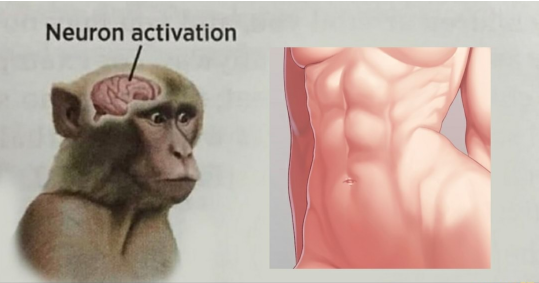
\includegraphics[height=6cm]{neuron_activation}
	\caption{A typical monkey's (maybe man also?) biological neural networks (BNN) gets activated by 2D{\tt/}anime girl's strong abs.}
\end{figure}

%------------------------------------------------------------------------------%

\section{Perception Learning Algorithm -- Thuật Toán Học Perceptron}

%------------------------------------------------------------------------------%

\section{Logistic Regression -- Hồi Quy Logistic}

%------------------------------------------------------------------------------%

\section{Softmax Regression -- Hồi Quy Softmax}

%------------------------------------------------------------------------------%

\section{Deep Neural Networks \& Backpropagation -- Mạng Neuron Đa Tầng \& Lan Truyền Ngược}

%------------------------------------------------------------------------------%

\section{Miscellaneous}

\subsection{Contributors}

%------------------------------------------------------------------------------%

\printbibliography[heading=bibintoc]
	
\end{document}